\label{SourceCodeAsTrees}
The sourcecode for a program needs to be read by the compiler, but also saved in some way so it is possible to manipulate the sourcecode, and performing the steps of the compiler.
This is done by using a tree.
The tree structure is good for this purpose because every node of the tree can contain different information, and have children which then makes it possible to express the productions of a grammar by following a path on the tree from the root to a leaf.
A Parse tree seperates the sourcecode into different productions from the grammar it represents, but also contains all of the syntax from the grammar, like parenthesis etc.
The tree structure also makes it possible to traverse the tree in the same path as the sourcecode is written, which means that the tree is able to express the structure of the sourcecode aswell as the statements which are found in the program.
An example of parse tree from the declaration \texttt{int a = 5;} can be seen on figure \myref{image:PST}

\begin{figure}
		\centering
	 	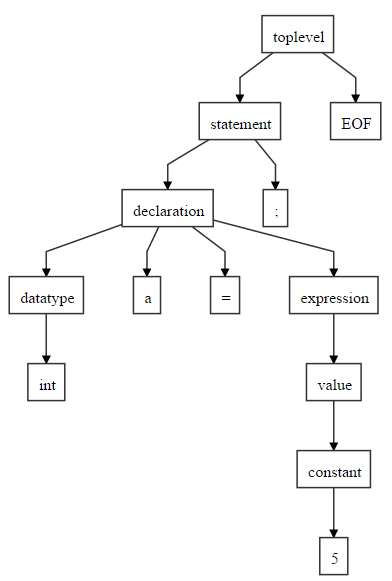
\includegraphics[width=0.6\linewidth]{figures/Trees/PST.PNG}
		\caption{A parse tree from the expression \texttt{int a = 5;} using the CFG for \gls{gamble}} \label{image:PST}
\end{figure}

The following chapter will explain how the compiler creates a parser to produce these parse trees for the sourcecode, and thus making it possible to use the trees in the compiler.
